\section{Experimentos e resultados} 

O algoritmo implementado é dependente principalmente de dois parámetros: alpha e número de iterações, por o que foram feitos alguns experimentos para saber quais são os melhores valores para cada um.
Para fazer os experimentos foi gerado um archivo de entrada com os seguintes parámetros:
	\begin{itemize}
		\item $N = 50$
		\item $M = 50$
		\item $T = 50$
		\item ${max}_{NC}$ = 20
	\end{itemize}
	Os experimentos foram feitos para os tres critérios mencionados em ~\ref{sec:criterios} e para todos os casos os elevadores tem capacidade 20. Os tempos de execução e os custos são comparados em cada um. Finalmente, a quantidade de execuções por experimento é 20 para todos os experimentos.

\subsection{Experimentos com Alpha}
\label{subsec:expalpha}
	Os experimentos nesta secção variaram o valor de alpha de 0.05 a 0.95 e tinham o valor de número de iterações igual a 100 para cada um dos tipos de custo. A continuação os resultados.
	\subsubsection{Para distancia}
		A figura~\ref{fig:costdistancealpha} mostra que o melhor valor tendo como custo a distancia (ou percurso total dos elevadores) é $\alpha = 0.45$. Além, tem um dos melhores tempos de execução como se mostra na figura~\ref{fig:timedistancealpha}
		\begin{figure}[H]
			\centering
			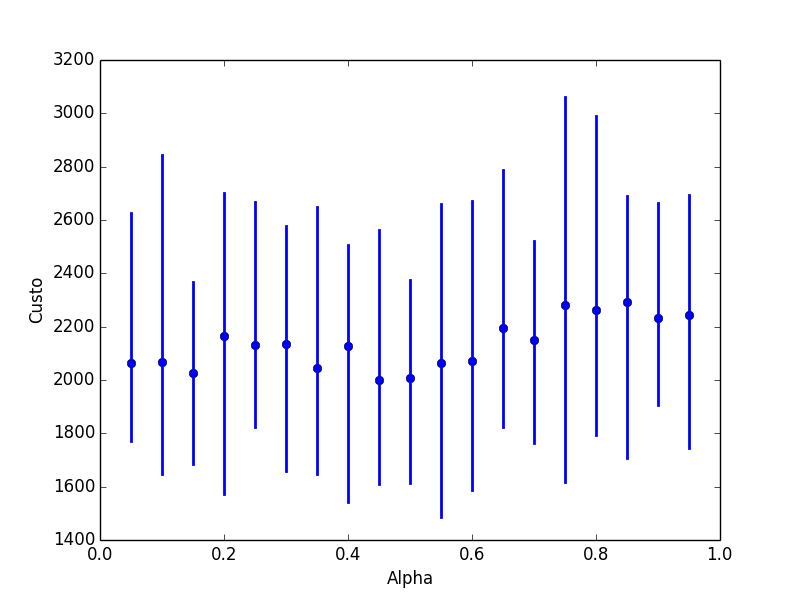
\includegraphics[height=8cm]{images/cost_distance_alpha}
			\caption{Custos com distancia}
			\label{fig:costdistancealpha}
		\end{figure}
		
		\begin{figure}[H]
			\centering
			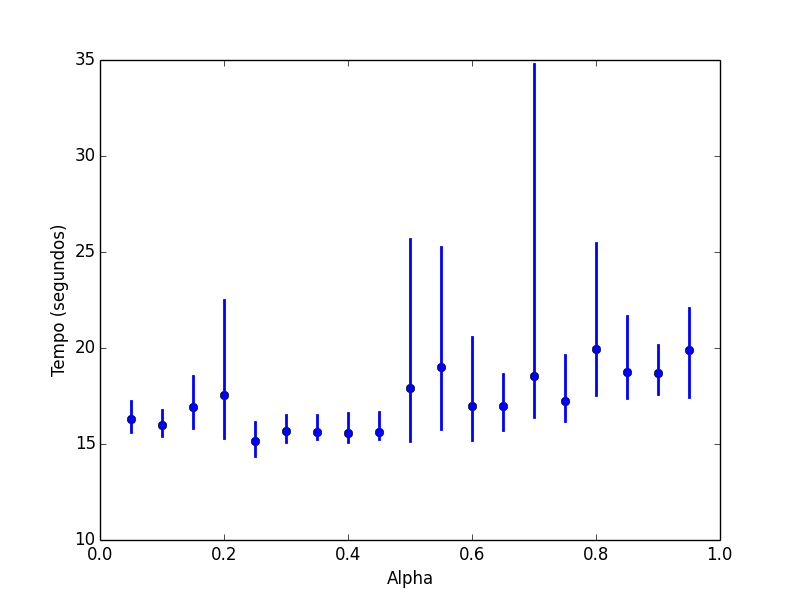
\includegraphics[height=8cm]{images/time_distance_alpha}
			\caption{Tempo com distancia}
			\label{fig:timedistancealpha}
		\end{figure}
		
	\subsubsection{Para tempo de espera e tempo no elevador}
		Neste experimento o melhor valor para alpha é $\alpha = 0.25$ como mostra a figura\~ref{fig:costwaitingalpha} e tem um bom tempo de execução comparado com os demais.
		\begin{figure}[H]
			\centering
			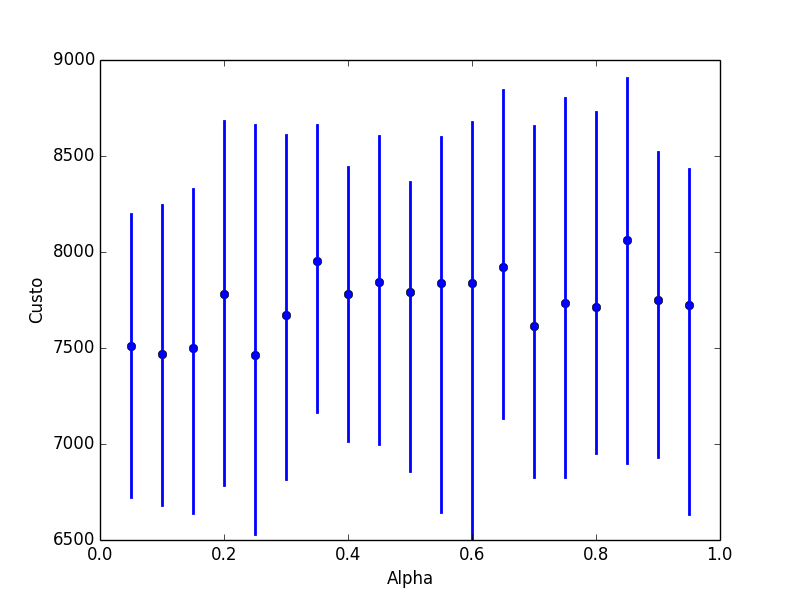
\includegraphics[height=8cm]{images/cost_waitingTime_alpha}
			\caption{Custos com tempo de espera e tempo no elevador}
			\label{fig:costwaitingalpha}
		\end{figure}
		
		\begin{figure}[H]
			\centering
			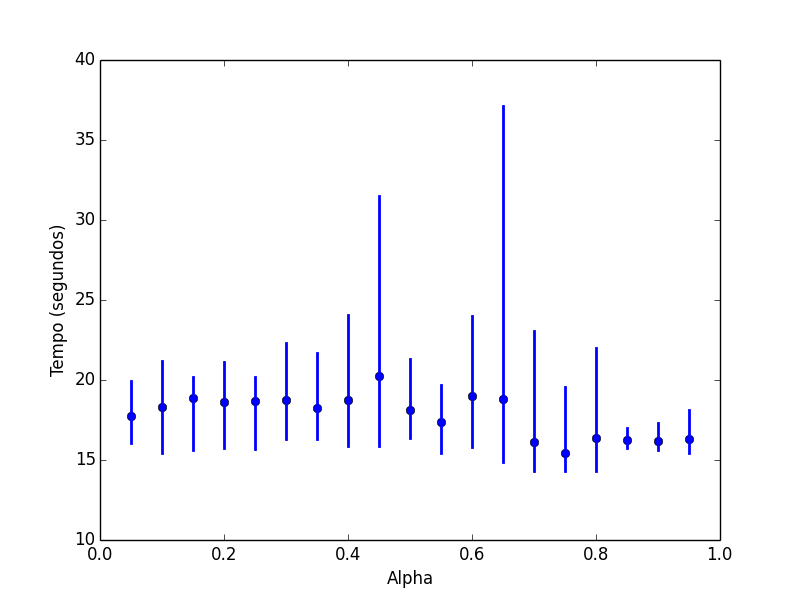
\includegraphics[height=8cm]{images/time_waitingTime_alpha}
			\caption{Tempo com tempo de espera e no elevador}
			\label{fig:timewaitingalpha}
		\end{figure}
	
	\subsubsection{Para ambos critérios}
		Por último, a figura~\ref{fig:costbothalpha} mostra que o melhor valor para usar com ambos critérios para calculo de custo é $\alpha = 0.4$ porque tem o menor valor para custo e também a melhor media, mas tem um dos maiores tempos de execução em promedio (ver figura~\ref{fig:timebothalpha}).
		
		\begin{figure}[H]
			\centering
			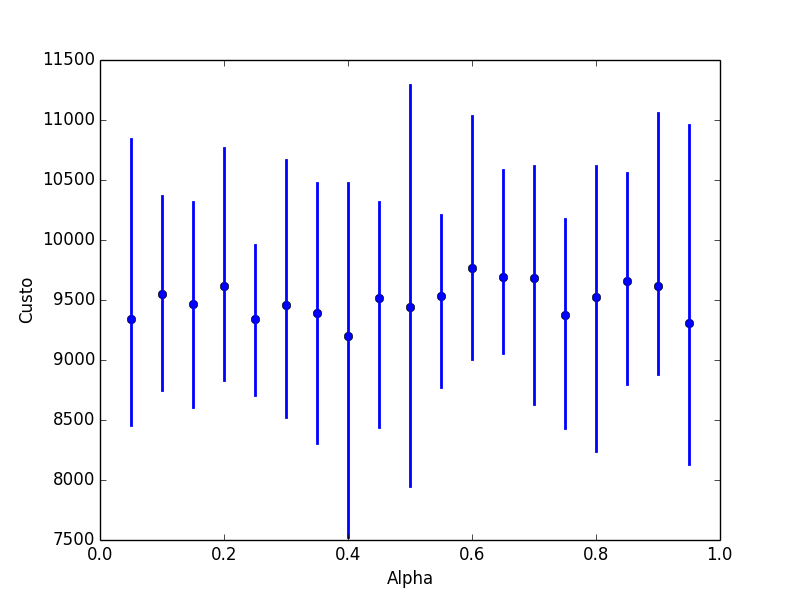
\includegraphics[height=8cm]{images/cost_both_alpha}
			\caption{Custos com ambos critérios}
			\label{fig:costbothalpha}
		\end{figure}
		
		\begin{figure}[H]
			\centering
			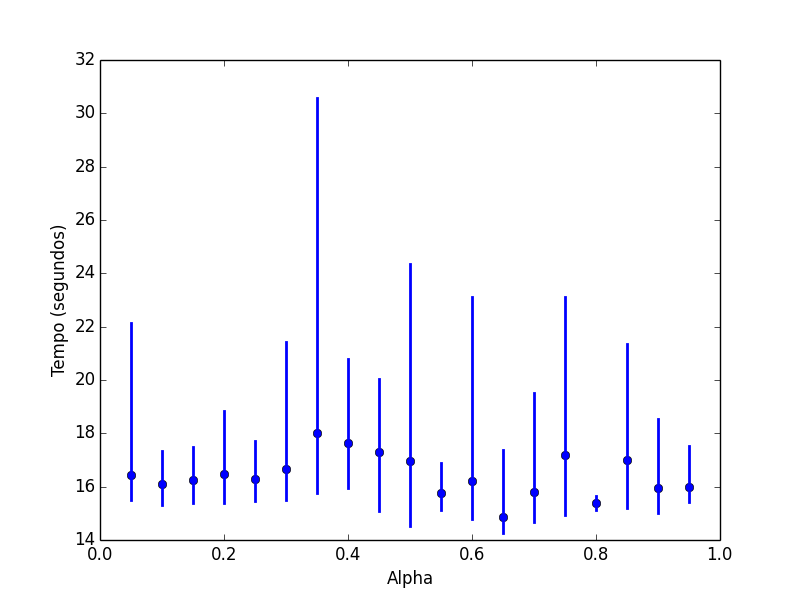
\includegraphics[height=8cm]{images/time_both_alpha}
			\caption{Tempo com ambos critérios}
			\label{fig:timebothalpha}
		\end{figure}

 \subsection{Experimentos com número de iterações}
 	Da mesma forma que em~\ref{subsec:expalpha} temos experimentos com o número de iterações, esta vez os valores de número de iterações variaram de 100 a 1000. Além, o valor de alpha foi o melhor valor resultado dos experimentos~\ref{subsec:expalpha}. A continuação os resultados.
 	\subsubsection{Para distancia} % FALTA
		\begin{figure}[H]
			\centering
			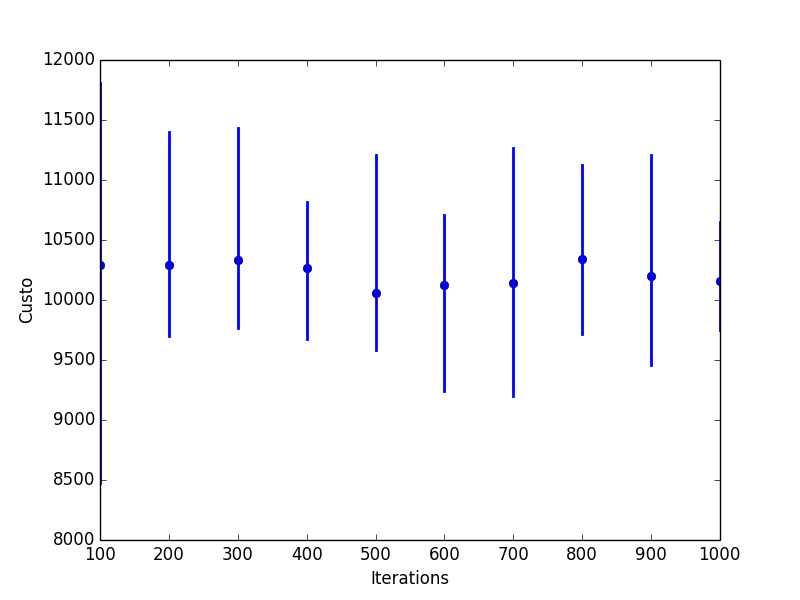
\includegraphics[height=8cm]{images/cost_both_iterations}
			\caption{Custos com distancia}
			\label{fig:costdistanceiterations}
		\end{figure}
		
		\begin{figure}[H]
			\centering
			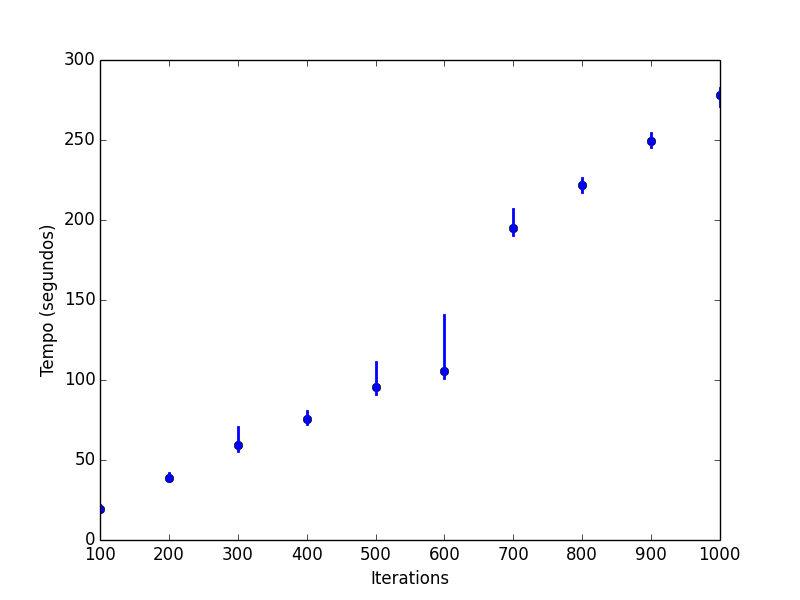
\includegraphics[height=8cm]{images/time_both_iterations}
			\caption{Tempo com distancia}
			\label{fig:timedistanceiterations}
		\end{figure}
	
	\subsubsection{Para tempo de espera e tempo no elevador} % FALTA
		\begin{figure}[H]
			\centering
			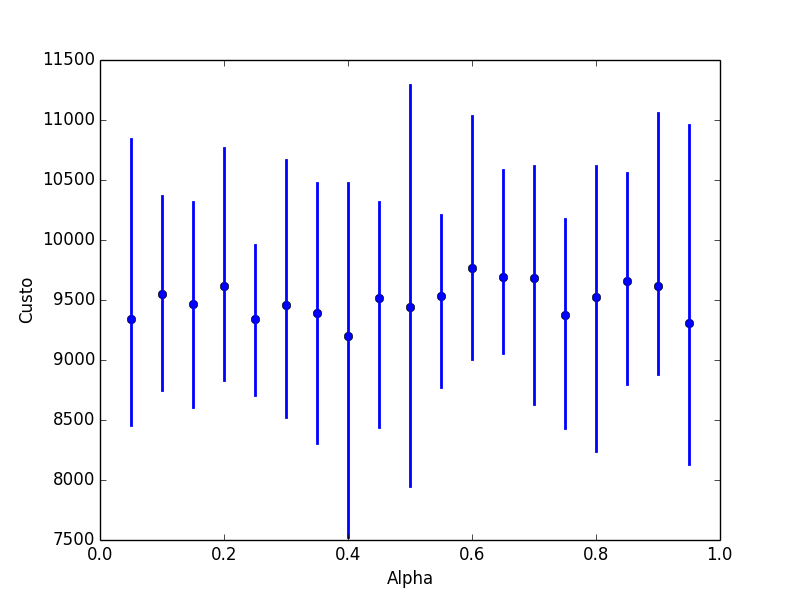
\includegraphics[height=8cm]{images/cost_both_alpha} % CAMBIAR
			\caption{Custos com tempo de espera e tempo no elevador}
			\label{fig:costwaitingiterations}
		\end{figure}
		
		\begin{figure}[H]
			\centering
			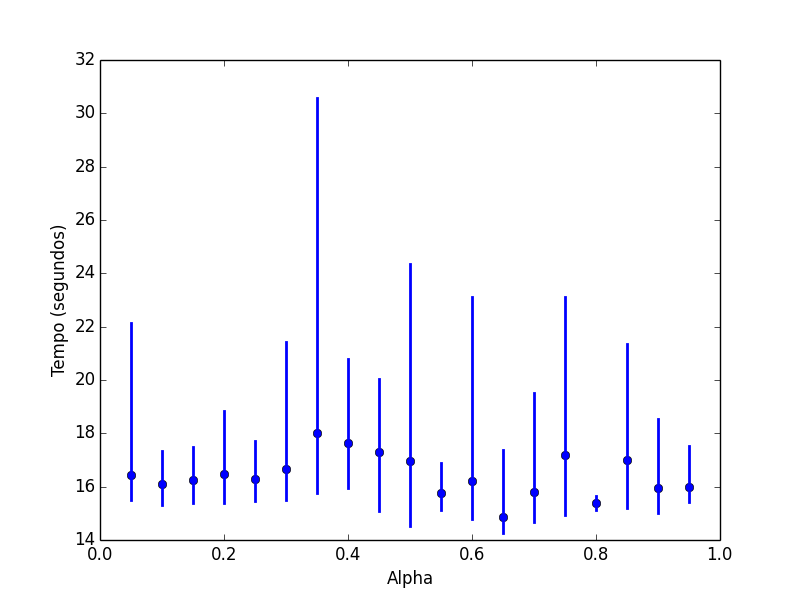
\includegraphics[height=8cm]{images/time_both_alpha} % CAMBIAR
			\caption{Tempo com tempo de espera e tempo no elevador}
			\label{fig:timewaitingiterations}
		\end{figure}
	
	\subsubsection{Para ambos critérios} % FALTA
		\begin{figure}[H]
			\centering
			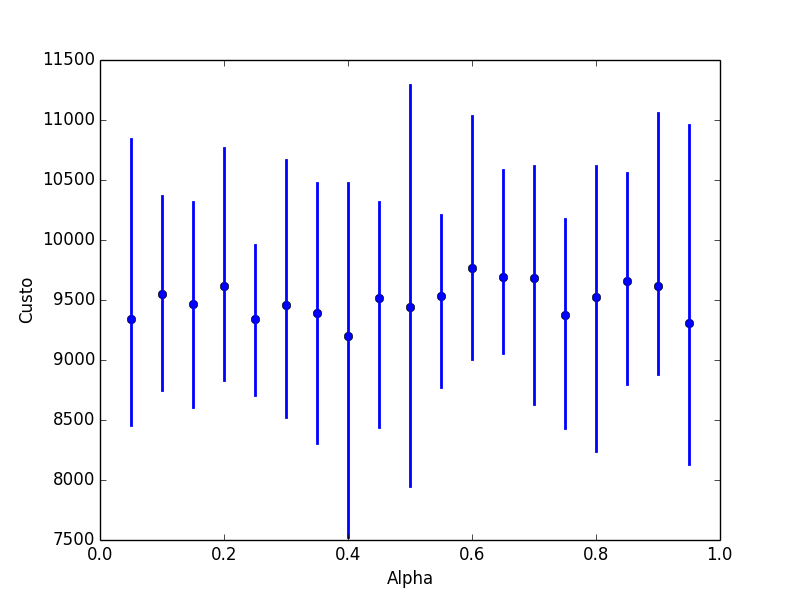
\includegraphics[height=8cm]{images/cost_both_alpha} % CAMBIAR
			\caption{Custos com ambos critérios}
			\label{fig:costbothiterations}
		\end{figure}
		
		\begin{figure}[H]
			\centering
			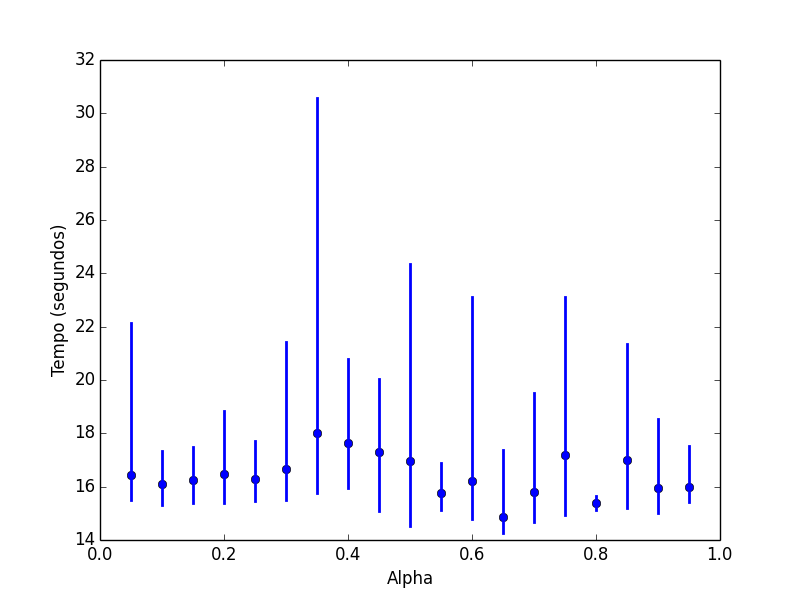
\includegraphics[height=8cm]{images/time_both_alpha} % CAMBIAR
			\caption{Tempo com ambos critérios}
			\label{fig:timebothiterations}
		\end{figure}